\begin{figure}[!htbp]
	\centering
	\resizebox{0.95\textwidth}{!}{%
		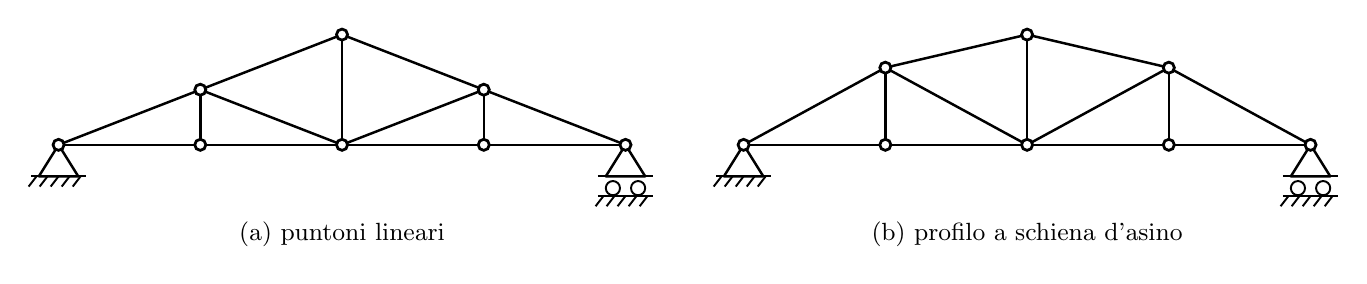
\begin{tikzpicture}[
			asta/.style={line width=0.90pt, line cap=round, line join=round, black},
			cord/.style={line width=0.90pt, line cap=round, line join=round, black},
			nodo/.style={circle, fill=white, draw=black,
				inner sep=0pt, minimum size=4pt, line width=1.0pt},
			terra/.style={line width=0.7pt, black},
			]
			\def\d{1.8}
			\def\hr{1.4}
			
			%% ── (a) puntoni lineari ────────────────────────────────
			\begin{scope}[xshift=0cm]
				\draw[cord](0,0)--(4*\d,0);
				\draw[cord](0,0)--(\d,{\hr/2})--(2*\d,\hr)--(3*\d,{\hr/2})--(4*\d,0);
				\draw[asta](2*\d,0)--(2*\d,\hr);
				\draw[asta](\d,0)--(\d,{\hr/2});
				\draw[asta](3*\d,0)--(3*\d,{\hr/2});
				\draw[asta](\d,{\hr/2})--(2*\d,0);
				\draw[asta](2*\d,0)--(3*\d,{\hr/2});
				\draw[cord](0,0)--(-0.25,-0.40)--(0.25,-0.40)--cycle;
				\draw[terra](-0.35,-0.40)--(0.35,-0.40);
				\foreach \xx in {-0.28,-0.14,0,0.14,0.28}
				\draw[terra](\xx,-0.40)--++(-0.10,-0.13);
				\draw[cord](4*\d,0)--(4*\d-0.25,-0.40)--(4*\d+0.25,-0.40)--cycle;
				\draw[terra](4*\d-0.35,-0.40)--(4*\d+0.35,-0.40);
				\draw[terra](4*\d-0.16,-0.55)circle(0.09);
				\draw[terra](4*\d+0.16,-0.55)circle(0.09);
				\draw[terra](4*\d-0.35,-0.65)--(4*\d+0.35,-0.65);
				\foreach \xx in {-0.28,-0.14,0,0.14,0.28}
				\draw[terra](4*\d+\xx,-0.65)--++(-0.10,-0.13);
				\foreach \x in {0,1,2,3,4} \node[nodo]at(\x*\d,0){};
				\node[nodo]at(\d,{\hr/2}){};
				\node[nodo]at(2*\d,\hr){};
				\node[nodo]at(3*\d,{\hr/2}){};
				\node[below,font=\small]at(2*\d,-0.85){(a) puntoni lineari};
			\end{scope}
			
			%% ── (b) profilo spezzato ───────────────────────────────
			\begin{scope}[xshift=8.7cm]
				\draw[cord](0,0)--(4*\d,0);
				\draw[cord](0,0)--(\d,{0.7*\hr})--(2*\d,\hr)--(3*\d,{0.7*\hr})--(4*\d,0);
				\draw[asta](2*\d,0)--(2*\d,\hr);
				\draw[asta](\d,0)--(\d,{0.7*\hr});
				\draw[asta](3*\d,0)--(3*\d,{0.7*\hr});
				\draw[asta](\d,{0.7*\hr})--(2*\d,0);
				\draw[asta](2*\d,0)--(3*\d,{0.7*\hr});
				\draw[cord](0,0)--(-0.25,-0.40)--(0.25,-0.40)--cycle;
				\draw[terra](-0.35,-0.40)--(0.35,-0.40);
				\foreach \xx in {-0.28,-0.14,0,0.14,0.28}
				\draw[terra](\xx,-0.40)--++(-0.10,-0.13);
				\draw[cord](4*\d,0)--(4*\d-0.25,-0.40)--(4*\d+0.25,-0.40)--cycle;
				\draw[terra](4*\d-0.35,-0.40)--(4*\d+0.35,-0.40);
				\draw[terra](4*\d-0.16,-0.55)circle(0.09);
				\draw[terra](4*\d+0.16,-0.55)circle(0.09);
				\draw[terra](4*\d-0.35,-0.65)--(4*\d+0.35,-0.65);
				\foreach \xx in {-0.28,-0.14,0,0.14,0.28}
				\draw[terra](4*\d+\xx,-0.65)--++(-0.10,-0.13);
				\foreach \x in {0,1,2,3,4} \node[nodo]at(\x*\d,0){};
				\node[nodo]at(\d,{0.7*\hr}){};
				\node[nodo]at(2*\d,\hr){};
				\node[nodo]at(3*\d,{0.7*\hr}){};
				\node[below,font=\small]at(2*\d,-0.85){(b) profilo a schiena d'asino};
			\end{scope}
			
	\end{tikzpicture}}
	\caption{Famiglie di maglie triangolari --- correnti spezzati
		(segue la \FIGref{fig:correnti_paralleli}).
		\emph{(d)}~Capriata a puntoni rettilinei: i nodi
		intermedi del corrente superiore giacciono sulla
		retta appoggio--colmo.
		\emph{(e)}~Profilo a schiena d'asino: i nodi
		intermedi sono al di sopra della retta di
		riferimento e il corrente superiore è
		genuinamente poligonale.}
	\label{fig:capriate_spezzato}
\end{figure}
